\documentclass[a4paper,titlepage,french]{report}
\usepackage[T1]{fontenc}
\usepackage[french]{babel}
\usepackage[utf8x]{inputenc}
\usepackage{amsmath}
\usepackage{eurosym}
\usepackage{float}
\usepackage{graphicx}
\usepackage[colorinlistoftodos]{todonotes}
\usepackage{placeins}
\usepackage{verbatim}
\usepackage{fmtcount}
\usepackage{array}
\usepackage[hidelinks]{hyperref}
\usepackage{url}
\usepackage[toc,page]{appendix} 
\renewcommand{\arraystretch}{1.25}

\usepackage{tabularx}
\newcounter{cptspec}
\setcounter{cptspec}{0}
 
\title{INSA de Rennes \\ Quatrième année Informatique \\ \bigskip \hrule \bigskip Rapport de conception \\ \bigskip Projet Value-at-Risk \bigskip \hrule}

\author{Benjamin \bsc{Bouguet} - Damien \bsc{Carduner} \\Paul \bsc{Chaignon} - Eric \bsc{Chauty} - Xavier \bsc{Fraboulet} \\ Clément \bsc{Gautrais} - Ulysse \bsc{Goarant} \\ ~~\\
Hamdi \bsc{Raissi} - Ivan \bsc{Le Plumey} \\ Quentin \bsc{Giai Gianetto}}


\date{Janvier 2014}

\begin{document}
\maketitle

\thispagestyle{empty}
\newpage

~~
\thispagestyle{empty}
\newpage

\tableofcontents
\newpage


\addcontentsline{toc}{chapter}{Introduction}
\chapter*{Introduction}

Ce rapport présente les modifications apportées au cours du projet aux rapports précédents.
Nous présentons aussi, en fin de ce rapport, l'état d'avancement des tests et la couverture actuelle.

Nous n'avons effectué qu'une seule modification des spécifications sous la contrainte du temps.
Les autres rectifications sont plus résultat de discussions avec notre encadrant qui prend le rôle de client.

Les rectifications pour la partie conception concernent essentiellement des changements dans les composants externes utilisés.
Nous avons du remplacer deux des librairies que nous comptions utiliser, l'une pour des soucis techniques et l'autre pour trouver un moyen plus simple.


\chapter{Modifications apportées}

\section{Spécifications}

\subsection{Importation et exportation}

Dans un soucis de respect des délais nous avons revu les fonctionnalités d'importation et d'exportation.
Cette modification concerne les spécifications S1, S2, S9 et S10 (respectivement l'importation et l'exportation d'actifs ainsi que l'exportation et l'importation de portefeuilles).

Nous avons fusionné ces fonctionnalités ensemble et l'utilisateur doit maintenant exporter l'entièreté de sa session.
De même, pour l'importation, il n'est plus possible de choisir les éléments à importer depuis l'archive sélectionnée.

La possibilité de choisir les éléments à exporter ou importer sera la première amélioration développée si les délais le permettent finalement.


\subsection{Gestion des portefeuilles}

Après plusieurs discussions avec notre encadrant nous avons décidé de modifier en profondeur la gestion des portefeuilles.

Tout d'abord, la restauration des portefeuilles supprimés ne constituant pas une priorité nous l'avons retiré des spécifications.

De plus, il apparaît que l'utilisateur ne sera que rarement amené à changer la constitution d'un portefeuille.
Il aura plutôt tendance à vouloir en créer un nouveau basé sur le premier.
Nous avons donc introduit la notion de parent pour un portefeuille et retiré les spécifications S6 à S8.

Ce changement ne réduit par le temps nécessaire pour développer la gestion des portefeuilles car la notion de parent amène de nouveaux problèmes de récurrence (notamment lors de la sauvegarde et de l'importation/exportation).


\subsection{Sauvegarde de la session}

Cette modification concerne la spécification S11.
Afin de simplifier l'implémentation les actifs sont directement enregistrés dans la base de données.
Lorsque l'utilisateur effectue une sauvegarde, il n'y a donc maintenant plus que les portefeuilles et leurs rapports qui nécessitent d'être sauvegardés.


\subsection{Matrice de corrélation}

La matrice de corrélation dont la génération est détaillée dans la spécification S20 fait maintenant partie du rapport de statistiques.
En effet, nous avons considéré que cette matrice faisait partie des informations générales sur le portefeuille et qu'elle a donc sa place dans le rapport de statistiques.


\section{Modélisations}

\subsection{Modélisation des rapports}

La modélisation - à la fois de la base de données et des classes - a été légèrement modifiée pour les rapports.
Nous avions prévu d'avoir un attribut pour chaque type de rapport.
Il est finalement plus simple d'avoir un seul attribut pour tous les types de rapport.
L'attribut désigne alors le nom des fichiers rapports sans leur extension.
Cette modification nous évitera également d'avoir à changer le modèle si nous souhaitons ajouter un nouveau type de rapport.


\section{Choix techniques}

\subsection{Interface avec R}

Nous avions décidé dans le rapport de conception d'utiliser la librairie RInside pour l'interfaçage entre notre code C++ et R.
Nous nous sommes cependant heurté à de nombreuses incompatibilités entre versions sous Windows.
La dernière version de RInside n'est pas complètement compatible avec Qt 5.0 \footnote{Or nous avons besoin de certaines fonctionnalités de cette dernière version de Qt, notamment pour importer et exporter au format JSON.}.

Après des échanges avec un des contributeurs au projet RInside et de nombreuses essais \footnote{Nous avons tenté de recompiler RInside avec différentes versions de MinGW sous les conseils du contributeur RInside.}, nous avons décidé d'abandonner l'usage de cette librairie pour effectuer à la place un appel direct du programme Rscript dans un nouveau processus.
Ce dernier permet tout simplement d'exécuter des scripts R depuis le terminal.


\subsection{Génération des rapports}

Pour générer les rapports DOCX nous avions décidé d'utiliser la librairie libopc. % TODO Ajouter ref.
Finalement cette librairie est assez compliquée à utiliser.
Elle présente un grand nombre de possibilités mais nécessite de la programmation bas niveau \footnote{Toujours en C++ mais très éloigné du code de Qt.}.

Comme nous n'avons pas besoin d'autant de possibilités nous avons préféré utiliser une librairie plus simple, écrite en Java, xdocreport. % TODO Ajouter ref.
Nous avons donc développé un petit programme qui permet, à partir d'informations au format JSON et d'un template de DOCX, de générer notre rapport aux format DOCX et PDF.
Ce programme permet donc d'utiliser les fonctionnalités de la librairie depuis la ligne de commande.

En effet, la librairie xdocreport permet d'écrire avec l'aide Word des \textit{templates} de rapport.
Certains champs spéciaux de ces \textit{templates} sont ensuite remplacés par les informations du document JSON.
Nous appelons ensuite, tout simplement, ce programme depuis notre logiciel avec les bons paramètres.
Le nouveau diagramme de classe pour la génération des rapports est visible en figure \ref{fig:class-diagram-report-generation}

\begin{figure}[h]
 	\center
  	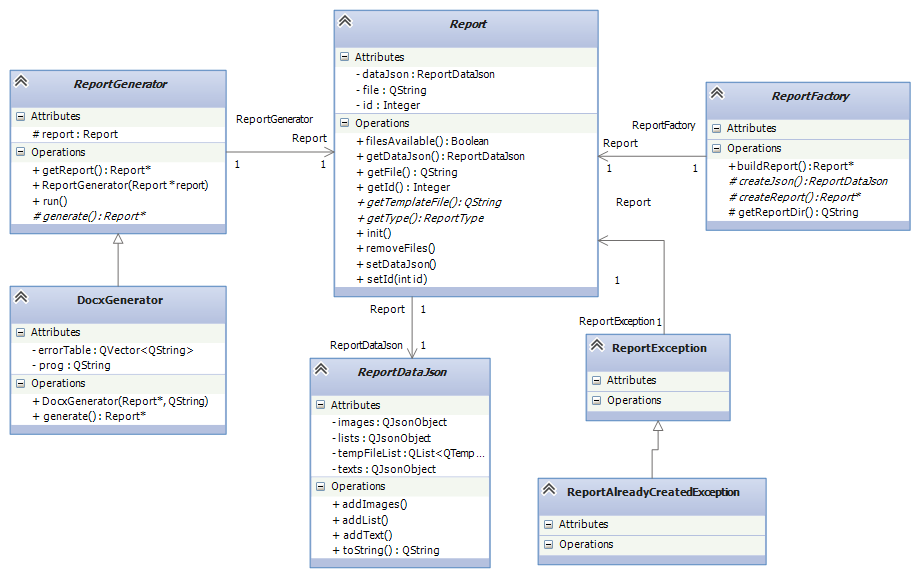
\includegraphics[scale=0.65]{class-diagram-report-generation.png}
  	\caption{Diagramme de classe de la génération des rapports}
	\label{fig:class-diagram-report-generation}
\end{figure}

Notre programme Java est suffisamment générique pour être utilisé dans d'autre logiciel.
Nous l'avons donc placé sous licence libre MIT. % TODO Ajouter ref.

Au vu du temps finalement économisé sur la génération des rapports, ce choix technique était judicieux.
De plus, notre programme Java est bien plus maintenable que ce que nous aurions pu développer avec la librairie libopc.


\chapter{Compte-rendu des phases de test}

\section{Intégration continue}

Nous avons décidé, dès le début de la phase de développement, de faire notre projet en intégration continue.
Cela signifie que chaque nouvelle fonctionnalité ou amélioration est développée sur une branche séparé, en parallèle de la branche principale.

Au moment de fusionner les deux, l'intégralité du nouveau code est relu par au moins un autre développeur.
Ce dernier doit alors s'assurer que la branche est bien couverte par de nouveaux tests unitaires (ou fonctionnels dans certains cas), effectuer quelques tests adaptés du logiciel manuellement et relire le code.
La relecture permet de signaler tout problème ou amélioration possible du code.

Pour cela nous avons utilisé le gestionnaire de versions git et le service d'intégration continue Travis CI qui s'intègre parfaitement dans GitHub.
Ce dernier nous permet notamment d'automatiser l'exécution de tous les tests automatisés à chaque commit ainsi qu'au moment de fusionner les branches.
Cela nous assure notamment de toujours maintenir la branche principale fonctionnelle.
Travis CI effectue aussi une rapide vérification des conventions de code à l'aide d'un script Python que nous avons développé.


\section{Tests fonctionnels}

Lors de la phase de conception nous prévoyons d'écrire les tests fonctionnels vers la fin de la phase de développement.
Finalement nous avons commencé à en écrire beaucoup plus tôt pour des raisons de simplicité.

En effet, certaines fonctionnalités utilisent des composants très dépendants entre eux et cela complique donc l'écriture de réel tests unitaires.
Par exemple, l'importation des rapports ne peut se faire sans avoir importés les portefeuilles correspondants précédemment.

Pour ces cas un peu particuliers \footnote{Cela concerne les fonctionnalités d'importation et d'exportation ainsi que la sauvegarde vers la base de données} nous avons décidé d'écrire des tests fonctionnels.
La couverture du code n'en est pas modifiée pour autant.
Cela a uniquement pour conséquence de compliquer le débogage lors des tests échouent.


\section{Tests unitaires}

De part notre méthode de travail décrite ci-dessus, nous avons toujours conservé un taux de couverture du code très satisfaisant.
Celui-ci s'est maintenu à environ 80\% tout au long du projet, en prennant en compte les tests fonctionnels décrit ci-dessus.


\section{Tests manuels}

Nous avions décidé de ne pas développer de tests automatiques de l'interface graphique pour des raisons de temps.
Nous avons donc à la place, au fur et à mesure du développement, défini des scénarios de tests manuels.

Chaque scénario a pour but de valider une ou plusieurs fonctionnalitées.
Nous les avons ensuite appliqués à toutes les branches susceptibles de faire régresser les fonctionnalités testées.


\section{Tests empiriques}

\subsection{Estimation du modèle GARCH}

Nous avions décris dans le rapport de conception un moyen de tester les résultats de notre modélisation GARCH.
Ce test sera effectué manuellement et est actuellement en cours de développement.
Il nécessite notamment de générer un ensemble de données à partir d'un modèle GARCH théorique à l'aide de R.


\subsection{Calcul de la Value-at-Risk à partir d'un modèle GARCH}

Nous avions aussi décris un second test empirique permettant de valider les calculs de la Value-at-Risk.
Ce test s'appuie sur la fonctionnalité de backtesting.
Or cette dernière est sur une branche sur le point d'être fusionnée avec la branche principale.
Nous effectuerons donc ce test dès que la branche aura été vérifiée et fusionnée.



\chapter*{Conclusion}

Nous avons quelques changements à effectuer dans les spécifications sous la contrainte du temps.
En effet, nous avions légèrement surestimé le temps que nous pouvions consacrer au projet \footnote{Ou sous-estimé les contraintes des autres cours et projets suivant le point de vue.}.

Cependant ces modifications restent très raisonnables et la plupart des changements sont liés à l'avancement du projet : en entrant plus dans les détails d'implémentation nous avons découvert des problèmes. Nous les avons résolu soit par de plus amples discussions avec le client \footnote{Dans notre cas notre encadrant.} et par des changements techniques \footnote{Notamment les changements des deux librairies libopc et RInside.}.

Notre méthode travail par intégration continue nous a permis de remplir les objectifs en matière de qualité logicielle.
Le choix de cette méthode était justifiée par la grande importance, pour notre client, d'avoir un logiciel fonctionnel et correctement testé.

Il nous reste encore quelques tests à effectuer mais cela était prévu dans la plannification pour les dernières semaines.
Nous avons donc, pour l'instant, rempli les objectifs de notre projet.


\end{document}